%%%%%%%%%%%%%%%%%%%%%%%%%%%%%%%%%%%%%%%%%%%%%%%%%%%%%%%%%%%%%%%%%%%%%%%%%%%%%%%%
% IEEE Robotics and Automation Letters (RA-L) format: the IEEEtran journal class,
% which is what the RA-L template uses. Six pages including figures and references;
% appendices count toward the limit. RA-L review is double-anonymous, so the author
% block stays anonymous and prior work by these authors is cited in the third person.
%%%%%%%%%%%%%%%%%%%%%%%%%%%%%%%%%%%%%%%%%%%%%%%%%%%%%%%%%%%%%%%%%%%%%%%%%%%%%%%%

\documentclass[letterpaper, 10pt, journal, twoside]{IEEEtran}

\usepackage{graphicx}
\usepackage{amsmath}
\usepackage{amssymb}
\usepackage{amsthm}
\usepackage{array}
\usepackage{booktabs}
\usepackage{enumitem}
\usepackage{algorithm}
\usepackage{algpseudocode}
\usepackage{tikz}
\usetikzlibrary{arrows.meta,calc,positioning,fit}

\newtheorem{lemma}{Lemma}
\newtheorem{proposition}{Proposition}


\renewcommand{\topfraction}{0.88}
\renewcommand{\bottomfraction}{0.7}
\renewcommand{\textfraction}{0.1}
\renewcommand{\floatpagefraction}{0.75}
\renewcommand{\dbltopfraction}{0.88}
\renewcommand{\dblfloatpagefraction}{0.75}
\setcounter{topnumber}{3}
\setcounter{dbltopnumber}{3}
\setcounter{totalnumber}{4}

\title{A Decentralized Speed Advisory System with Global Traffic Awareness and Local Visual Sensing}

\author{Anonymous Authors%
\thanks{Anonymous affiliations.}%
}

\markboth{IEEE Robotics and Automation Letters. Preprint Version. Under Review}{Anonymous: A Decentralized Speed Advisory System}

\begin{document}
\maketitle

\begin{abstract}
Preventing traffic breakdown requires controlling vehicle arrivals before a bottleneck exceeds its critical density. Yet infrastructure-free control faces a sensing tradeoff: commercial probe feeds describe the road network but arrive late, whereas onboard cameras observe nearby vehicles with low latency but limited range. This paper presents a decentralized speed advisory system that combines these sources without roadside instrumentation, inter-vehicle communication, or a central speed coordinator. Each equipped vehicle independently computes a network-wide speed plan from a versioned traffic feed and applies it at a version-specific time; local visual occupancy estimates permit a gated, one-step downward correction. We characterize when delayed feed observations cannot support pre-breakdown intervention and derive a conditional sampling-margin bound for local sensing. A US\$500 phone-and-Jetson prototype was operated on public roads to characterize sensing, computation, and communication, and 18,818 recorded frames informed the simulated camera model; drivers did not follow the advisories during these drives. Across five disturbances in a Mainz-network simulation, the system prevented 55 of 74 jams that occurred without control, reduced mean jam time from 130.8 to 3.9 segment-minutes, increased throughput by 3.9\%, and reduced vehicle-hours in the network by 12.6\%. The results establish the potential of complementary global and local sensing for infrastructure-free preventive traffic control, subject to driver compliance and the simulated setting.
\end{abstract}

\section{Introduction}
\label{sec:intro}

\begin{figure}[t]
\centering
\begin{minipage}[b]{0.31\linewidth}\centering
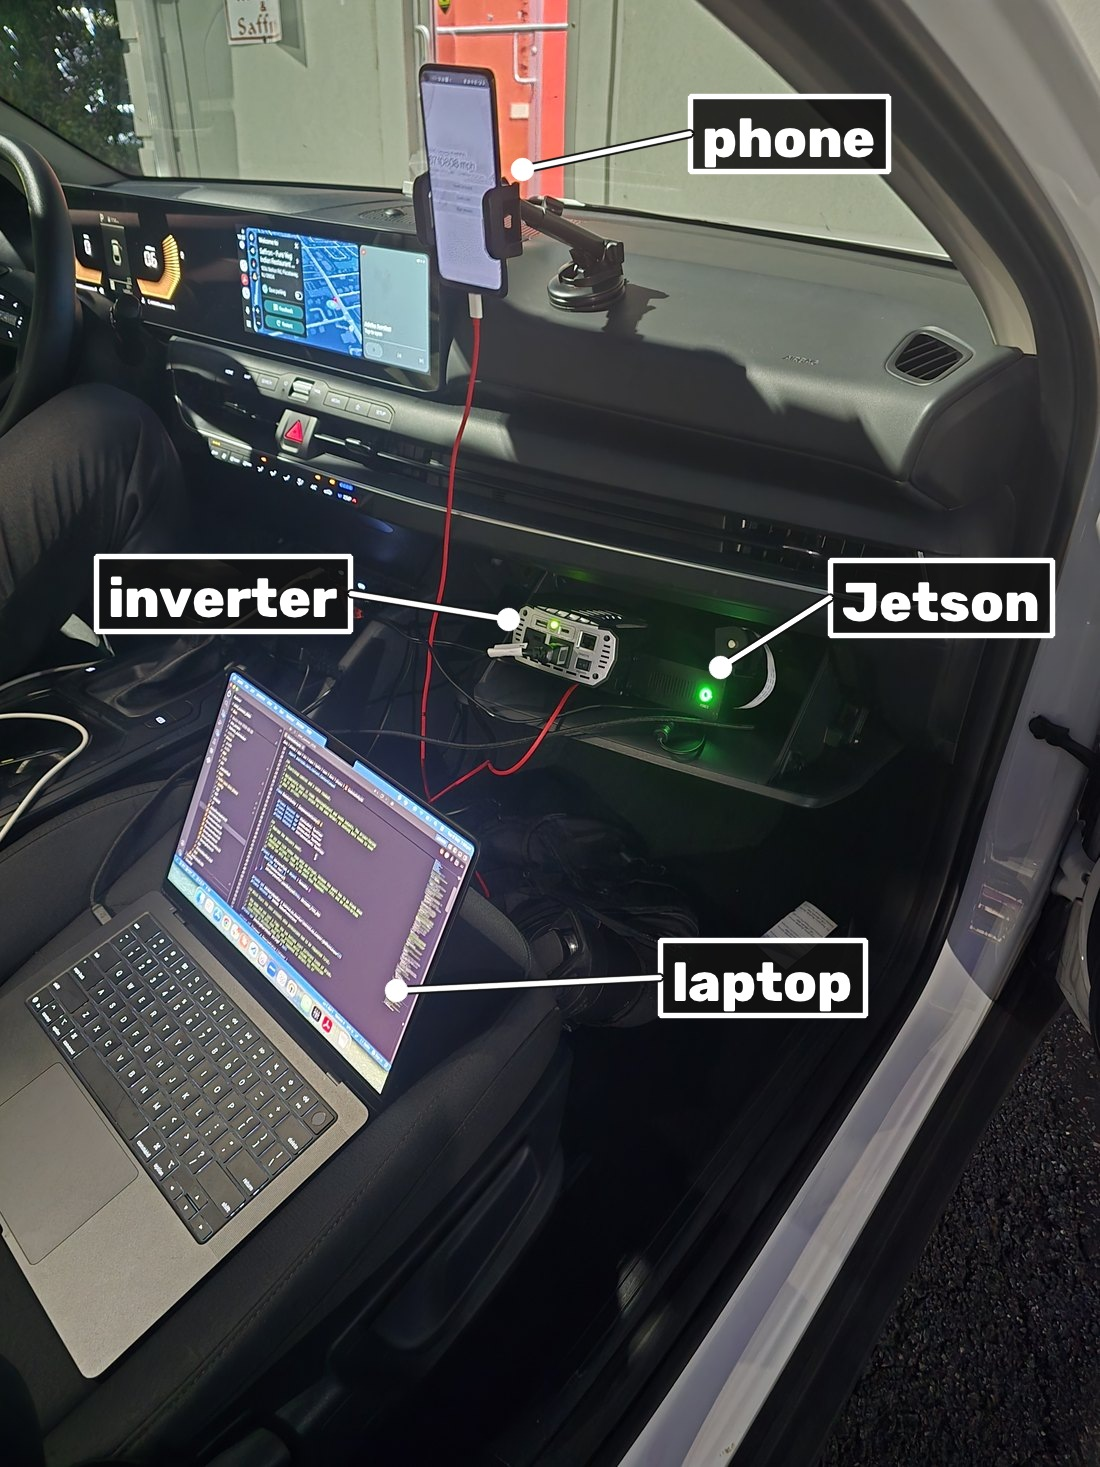
\includegraphics[height=1.33in]{images/rig_dashboard.jpg}\\[1pt]
{\footnotesize (a) The rig.}
\end{minipage}\hfill
\begin{minipage}[b]{0.66\linewidth}\centering
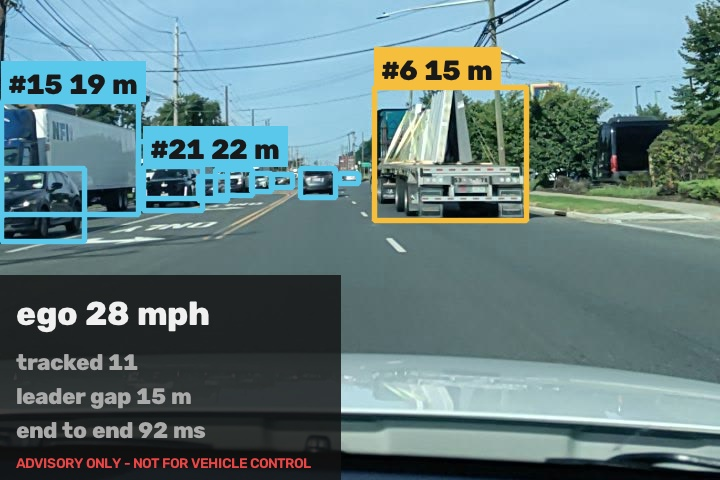
\includegraphics[height=1.33in]{images/perception_drive_frame.jpg}\\[1pt]
{\footnotesize (b) The local layer's view on a drive.}
\end{minipage}
\caption{The deployed system. In (a), the phone supplies the camera, GPS and inertial unit and carries the display; the Jetson runs perception, both advisory layers and the safety filter; the inverter is its only connection to the car. In (b), the leader in the ego lane is amber and the other tracked vehicles are cyan. Nothing connects to the throttle, the brakes, the steering or the vehicle bus.}
\label{fig:teaser}
\end{figure}

Traffic flow near capacity is vulnerable to short-lived disturbances. A temporary lane obstruction or an upstream inflow surge can raise density beyond the critical regime, reduce discharge flow, and produce a queue that persists after the disturbance ends~\cite{bhardwaj2023understanding}. When arrivals continue to exceed the reduced discharge rate, clearing an established queue is substantially harder than preventing its formation. Effective intervention must therefore influence vehicle arrivals \emph{before} breakdown.

Existing approaches regulate bottleneck inflow using roadside detectors and actuators, including ramp meters and variable speed limits~\cite{papageorgiou2002freeway,hegyi2008specialist}, or coordinate equipped vehicles through a centralized planner~\cite{lee2024traffic}. These approaches demonstrate the value of anticipatory control but depend on infrastructure, centrally maintained coordination, or instrumented fleets. A speed advisory delivered through an ordinary driver's phone offers a lower-modification alternative, although its effectiveness still depends on adoption and compliance.

Such an advisory must contend with complementary sensing limitations. Commercial probe feeds cover a road network but aggregate traffic conditions and report them with delay: prior measurements found a mean 4.4-minute latency for reported speed changes~\cite{wang2018latency}. The feed studied here publishes nominally once per minute and becomes readable 29--90\,s after the publication stamp. Conversely, an onboard camera can detect nearby spacing changes before a substantial speed drop but observes only roughly 60\,m of roadway. Neither source alone offers both network-scale anticipation and rapid detection at the vehicle.

The proposed system separates these roles (Fig.~\ref{fig:overview}). A \emph{global layer} maps each traffic-feed version to a network-wide speed plan. Because vehicles poll independently, computing the same plan is insufficient for agreement at the same instant; a version-keyed application time aligns plan changes without vehicle-to-vehicle messages or a server that computes individual advisories. A \emph{local layer} estimates occupancy and its recent trend from onboard video, applying at most one downward speed step when the road ahead approaches critical occupancy. A feed-based gate limits unnecessary corrections during otherwise uncongested conditions, and a safety filter constrains the displayed advice. The driver remains responsible for vehicle control.

Public-road tests of a phone-and-Jetson prototype informed the simulation camera model without testing driver compliance. In the Mainz network~\cite{self_regulating_cars}, the system prevented 55 of 74 jams, but reduced throughput by 3.0\% without a disturbance and remained sensitive to compliance.

\noindent\textbf{Contributions.} We present (i) version-keyed decentralized advisories with bounded camera corrections (Section~\ref{sec:controller}); (ii) measurements and conditional bounds for delayed feed and sampled visual sensing (Section~\ref{sec:feed}); (iii) an on-road prototype and camera error model from 18,818 frames (Section~\ref{sec:road}); and (iv) five-disturbance simulation ablations including compliance and unnecessary-intervention costs (Section~\ref{sec:eval}).


\section{Related Work}
\label{sec:related}

\noindent\textbf{Infrastructure-based prevention.} Ramp metering~\cite{papageorgiou2002freeway,arnold1998ramp} and variable speed limits~\cite{hegyi2008specialist,li2017reinforcement} regulate arrivals at bottlenecks using roadside measurements and controls. Integrating floating-car probes and video with variable speed limits has also improved detection and control in simulation~\cite{hegyi2013cooperative}. Their infrastructure dependence motivates vehicle-based alternatives.

\noindent\textbf{Vehicle-based traffic control.} Controlled vehicles can attenuate stop-and-go waves~\cite{stern2018dissipation}, and reinforcement learning has been explored for mixed-autonomy traffic~\cite{wu2017flow,vinitsky2018benchmarks,kreidieh2018dissipating}. Coarse speed advisories can influence human-driven vehicles~\cite{cho2023temporal}; CIRCLES demonstrated traffic control with approximately one hundred vehicles under centralized speed planning~\cite{lee2024traffic}. Here, onboard advisories use commercial observations without modifying vehicle controls; compliance is evaluated only in simulation.

\noindent\textbf{Delayed shared information.} Commercial probe observations cover large networks~\cite{herrera2010evaluation,seo2017traffic} but can lag physical changes by minutes~\cite{wang2018latency}. Shared observations can also support decentralized decisions without direct messages~\cite{nayyar2013common}; however, vehicles retrieving versions at different times may temporarily disagree even when using identical policies. Version-keyed application addresses this mismatch; visual sensing can warn earlier than feed-reported speed.


\section{Method}
\label{sec:method}

\subsection{System Overview}
\label{sec:system}

\begin{figure}[t]
\centering
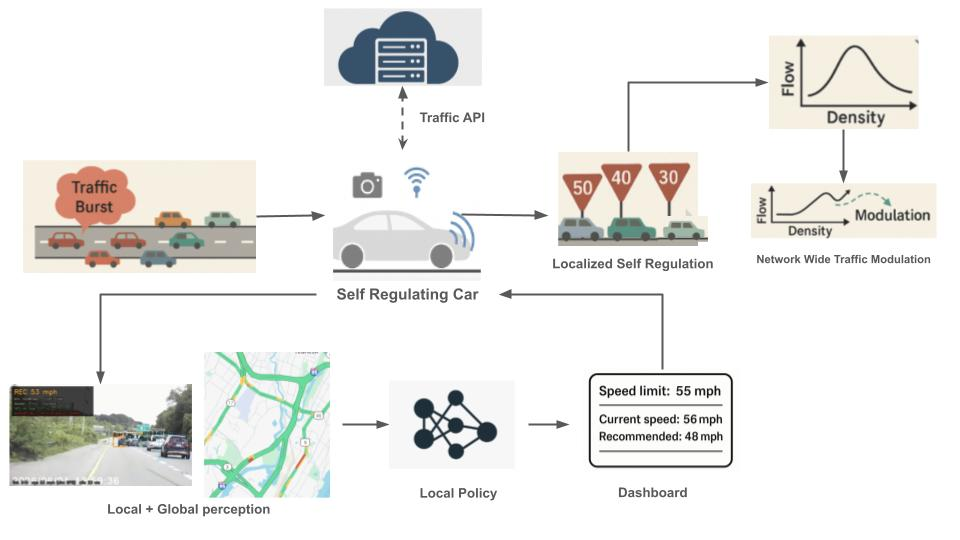
\includegraphics[width=0.9\linewidth]{images/system_overview.jpg}
\caption{System overview. A burst of inflow pushes a stretch of road toward its critical density. Each equipped vehicle reads the network from a commercial probe feed (global layer) and the road ahead from its own camera (local layer), computes its advisory onboard, and shows the driver a recommended speed. The vehicles coordinate only through the feed version they read; none talks to another.}
\label{fig:overview}
\end{figure}

\noindent\textbf{Design goals.} Preventive control must satisfy G1--G2 under the deployment constraints G3--G5.
\begin{itemize}[wide=0pt,itemsep=1pt,topsep=2pt]
\item[(G1)] \emph{See the whole network.} A segment jams because of vehicles that entered upstream of it, so advice that prevents the jam must reach them before they arrive, from the state of segments they have not yet reached.
\item[(G2)] \emph{Act before the road breaks down.} Near capacity a jammed bottleneck serves less traffic than keeps arriving, so the jam does not drain until demand falls (Section~\ref{sec:feed}); a controller that acts while the road still flows can keep the jam from forming.
\item[(G3)] \emph{Give consistent advice without a coordinator or messages between vehicles.} Inconsistent advisories can introduce undesirable speed differences between nearby participants. Plan agreement must not require direct inter-vehicle messaging~\cite{kenney2011dedicated,sae2020j2735} or a continuously available speed-coordination server.
\item[(G4)] \emph{Advise without touching the vehicle's controls.} Taking over the throttle or brakes requires modifying and certifying the vehicle, as for the CIRCLES vehicles~\cite{lee2024traffic}; an advisory fits any car and leaves the driver in control.
\item[(G5)] \emph{Run on hardware a driver can buy.} The system acts only through equipped vehicles, so the cost of equipping one limits how many take part; the rig of Section~\ref{sec:road} costs US\$500.
\end{itemize}

\begin{table}[t]
\centering
\caption{The two sources of information, as measured in this work.}
\label{tab:sources}
\footnotesize
\setlength{\tabcolsep}{4pt}
\begin{tabular}{@{}lll@{}}
\toprule
 & Feed (global layer) & Camera (local layer) \\
\midrule
Coverage & every network segment & 60\,m, own and side lanes \\
Measures & segment speed, jam factor & gaps, vehicles in range \\
Update & one version per 60\,s & every 5\,s \\
Delay to act & 99.5\,s & about 6\,s \\
Sees a jam when & speed has fallen & density is rising \\
\bottomrule
\end{tabular}
\end{table}

\noindent\textbf{One layer per source.} Neither source by itself meets G1 and G2 (Table~\ref{tab:sources}): the feed covers the network but reports a forming jam late, and the camera reports it early but sees only the next 60\,m. The global layer therefore sets a plan for the whole network from the feed, and the local layer may lower one vehicle's speed below that plan when its own camera sees the road filling. A subsequent safety filter limits advisories that are substantially below surrounding traffic speed and withholds advice when the available headway or time-to-collision falls below its minimum. 

\noindent\textbf{Inputs and outputs.} The network is divided into super-segments, twelve on the network we evaluate. For each, the global layer reads three fields from the HERE Traffic API~\cite{here_traffic_api}, \texttt{speed}, \texttt{free\_flow} and \texttt{jam\_factor}, and two from the map, lane count and length. Because the HERE jam-factor computation is not publicly specified, the simulation uses the approximation $\operatorname{clip}_{[0,10]}[10(1-v/v_f)]$, motivated by the travel-time-relative-to-free-flow formulation in~\cite{auxer2007rating}, where $v$ and $v_f$ denote observed and free-flow speeds. Each output is 0.5, 0.75, or 1.0 of the static speed limit, avoiding dependence on live speed readings.


\subsection{The Global-Local Speed Advisory}
\label{sec:controller}

\noindent\textbf{Global layer: a deterministic plan from shared observations.} Identical policies do not ensure simultaneous plans when vehicles poll independently. Each vehicle applies deterministic policy $\pi$ to a feed version, producing speed fractions for twelve super-segments. Trained by Q-learning on five feed/map fields per super-segment, it adapts the action set and speed--density reward of~\cite{self_regulating_cars} to feed observations. Identical versions yield identical plans~\cite{nayyar2013common}, yet retrieval times differ. To address it, vehicles apply a version at its stamped time plus a common delay $D$ (Algorithm~\ref{alg:agreement}). If clocks agree and polling succeeds within the measured maximum delivery lag, a delay $D$ at least that lag plus the polling interval allows every vehicle to retrieve the version. Unlike common-time polling, it tolerates the measured 26--34\,s publication-phase shifts without messaging.

\begin{algorithm}[t]
\caption{Version-keyed plan, run on every vehicle}
\label{alg:agreement}
\begin{algorithmic}[1]
\State query the feed every $P_q$ seconds, at the vehicle's own phase
\State on a response stamped $T$ newer than the held one: compute the plan $a=\pi(x)$
\State apply $a$ from $T+D$, or at once if $T+D$ has passed
\end{algorithmic}
\end{algorithm}

\noindent\textbf{Local layer: a one-step correction from the camera.} Every 5\,s the local layer estimates the occupancy $\hat k$ of the road ahead, the fraction of lane length that vehicles cover: in its own lane from the gap $s$ to the leader, as $L/(s+L)$ with $L=4.5$\,m, and in each lane beside it from the number $n$ of vehicles seen within the camera's effective range $R$, as $nL/R$; $\hat k$ is the mean over the visible lanes. The layer fits the trend $\dot k$ of $\hat k$ over the last 30\,s and computes the margin to the critical occupancy $k_c$,
\begin{equation}
M=\bigl(k_c-\hat k-\tau\max(\dot k,0)\bigr)/k_c,
\label{eq:margin}
\end{equation}
with $k_c=0.178$ and horizon $\tau=10$\,s. When $M\le 0$ the vehicle shows the next lower speed fraction instead of the plan's. The correction holds for at least 30\,s and releases once $M\ge 0.05$ on two consecutive samples, to reduce switching caused by noisy occupancy estimates. The horizon $\tau$ accounts for sampling and subsequent response time, including modeled driver reaction. Proposition~\ref{prop:margin} (\S\ref{sec:feed}) motivates using a predictive margin; it does not guarantee that the advisory immediately arrests occupancy growth.

\noindent\textbf{When the correction may act.} The camera sees only the next 60\,m, and near capacity ordinary traffic also brings the occupancy ahead close to $k_c$, so a correction without a gate slows vehicles that did not need slowing. A feed gate therefore lets the correction switch on only while the feed version the vehicle applies shows a jam factor of at least $J_g=1$ on some super-segment, measured against one step below that version's plan so that the advisory's own slowing does not read as congestion. Every vehicle that applies the same version sees the same gate, and a corrected vehicle is released through the hysteresis when its gate closes.

\noindent\textbf{Why the correction is asymmetric and bounded.} A vehicle that sees an empty road ahead does not know that the network downstream is filling, which the plan does know, so it must not speed up; a vehicle that sees a filling road needs only to slow its own arrival, and the single-step restriction bounds the difference from the shared plan and is intended to reduce the risk of introducing an excessively slow vehicle. This bound limits advisory differences but does not guarantee their traffic effect.


\section{Timing Analysis of Jam Prevention}
\label{sec:feed}

\noindent\textbf{Measured publication and delivery delays.} A feed version's publication stamp does not mark when vehicles can use it: delayed availability can leave independently polling vehicles on different plans. To quantify this gap, we polled feeds over Mainz and New Jersey every 5\,s for 1.9 hours. Mainz published 113 versions 60\,s apart, readable 34.4--89.5\,s after their stamps. New Jersey showed publication-phase shifts, intervals as short as 28\,s, and lags of 28.9--84.0\,s; the 123 responses recorded during road drives were 34--110\,s old. We therefore schedule application $D=\bar L+P_q$ after the publication stamp, where $\bar L$ is the maximum measured delivery lag and $P_q$ the query interval. For Mainz, $D=99.5$\,s, enabling consistent application under the assumed delivery bound but adding delay to the probe latency itself~\cite{wang2018latency}.

\noindent\textbf{The lag condition.} Let $t_v$ be the first time a segment's speed departs from what it would have been without the triggering event, $t_{\mathrm{on}}$ the onset of the jam, and $W=t_{\mathrm{on}}-t_v$ the warning the speed signal gives. Every version stamped before $t_v$ is the same with and without the event.

\begin{proposition}[Lag condition]\label{prop:lag}
Let feed versions be published at most $g$ seconds apart and applied $D$ seconds after their stamps, and let no version stamped before $t_v$ depend on the event. Then a controller that reads only the feed cannot change an advised speed in response to the event before $t_v+D$, so it changes none before onset if $W<D$. If $D\le W<D+g$ and the stamp phase is uniform, it acts before onset with probability $(W-D)/g$.
\end{proposition}

\begin{proof}[Proof sketch]
The first stamp at or after $t_v$ falls in $[t_v,t_v+g)$ and is applied in $[t_v+D,t_v+D+g)$; nothing applied earlier differs from the case without the event. Acting before onset needs that stamp in $[t_v,t_{\mathrm{on}}-D)$, an interval of length $W-D$ out of $g$.
\end{proof}

This is a necessary, not sufficient, condition: drivers must also respond before onset. The interval $W$ can be short because speed may change little on the free-flow branch even as density rises. An occupancy estimate derived from local vehicle gaps can therefore offer earlier warning.

\noindent\textbf{How often the local layer must sample.} A rule that observes density only at sample instants protects the critical density only if it acts early enough to absorb the rise that can happen before its next action.

\begin{proposition}[Sampled margin]\label{prop:margin}
Let local density rise no faster than $r$, let a rule sample it every $\Delta$ and act $l$ after a sample, and let its action stop the rise. If the rule acts at the first sample at or above $k^\ast-r(\Delta+l)$, density stays below $k^\ast$.
\end{proposition}

\begin{proof}[Proof sketch]
The sample before the one that triggers the action was below $k^\ast-r(\Delta+l)$, and density rises by at most $r(\Delta+l)$ before the action.
\end{proof}

For the feed, $\Delta+l$ is $60\,\mathrm{s}+D$, about 160\,s on the Mainz process; for a camera sampled every 5\,s with about 1\,s of processing it is 6\,s. Under these idealized assumptions, the camera's response horizon is over 25 times shorter; this does not guarantee that advice arrests occupancy growth.

\noindent\textbf{The role of reduced bottleneck discharge.} A point-queue approximation illustrates why breakdown prevention can be more effective than attempting to discharge an established queue.

\begin{proposition}[Point-queue drain]\label{prop:drain}
A queue of $Q$ vehicles with arrival rate $\lambda$ and service rate $\mu$ empties after $Q/(\mu-\lambda)$ if $\mu>\lambda$ and never otherwise. If the bottleneck serves $\mu_f$ before it breaks down and $\mu_q<\mu_f$ after, and $\mu_q\le\lambda<\mu_f$, no queue forms while it has not broken down, and none drains once it has.
\end{proposition}

On the Mainz network the jammed exit serves 3,535\,veh/h under no control, 37\,veh/h less than the background demand of 3,572\,veh/h, so a jam that forms there never drains, and preventing the breakdown is worth more than draining the queue faster.


\section{Implementation and On-Road Deployment}
\label{sec:road}

\noindent\textbf{Hardware and software.} The US\$500 rig combines a OnePlus Nord N10 phone (US\$150), Jetson Orin Nano (US\$250), and US\$100 of mounts, inverter, and cables (Fig.~\ref{fig:teaser}). The phone supplies video, GPS, inertial measurements, traffic updates, and display; the Jetson runs YOLOv8n~\cite{redmon2016yolo} detection at 640\,px, tracking, occupancy estimation, both advisory layers, and the safety filter. USB transfers inputs to the Jetson, keeping computation off the thermally constrained phone. Neither a vehicle-bus connection nor an advisory server is required.

\noindent\textbf{Road drives.} Eight public-road runs in central New Jersey on 2026-09-08 assessed whether the sensing and advisory pipeline could operate outside the laboratory. Over 152.8 minutes, the rig recorded 22{,}929 ticks, with valid GPS on 99.1\%, and received 123 successful feed responses. Two runs applied adaptive sampling, while six only logged the scheduler's decisions. These runs validate the sensing pipeline, not traffic effects: an approved human-participant study was outside their scope, so drivers did not follow advisories. Traffic outcomes are therefore evaluated in simulation (\S~\ref{sec:eval}).

\noindent\textbf{Latency and operational reliability.} Median detection-to-advisory latency was 19.8\,ms; USB reduced 95th-percentile transfer latency from 215.63 to 116.19\,ms. Despite these low latencies, operating conditions limited reliability. Direct sunlight pushed the windscreen-mounted phone into Android's severe thermal tier and closed the application on the first drive; a cable failure and a sunlight-disabled hotspot interrupted two others. Thermal management and connectivity, rather than inference speed, remain practical constraints.

\noindent\textbf{From road video to simulated observations.} The road recordings also let the simulation capture two distinct limitations of monocular sensing: missed vehicles at longer range and uncertain distances to those detected. We processed 18,818 synchronized frames from six drives with the deployed detector, tracker, and distance estimator, deriving error tables from the four drives recorded at five frames per second. Against a 1,280\,px reference pass, not ground truth, detection fell from 0.95 within 10\,m to 0.53 at 40--50\,m and 0.32 at 50--60\,m. Accordingly, the simulated camera has a 60\,m effective range and occlusion by nearer vehicles. Bounding-box-width distances include frame noise increasing from 0.05\,m at 10\,m to 1.1\,m at 50--60\,m, plus a persistent per-vehicle offset with 31\% spread from vehicle-width variation. The phone's unrecorded focal length leaves the absolute distance scale assumed; Section~\ref{sec:sens} tests its effect.

\section{Evaluation in Simulation}
\label{sec:eval}

\subsection{Testbed and Protocol}
\label{sec:sim}

\begin{table}[t]
\centering
\caption{Ablation over seeds 16--30: five triggers (75 runs) and no trigger (15 runs). Jam-free: runs with no jam. Jam: jammed segment-minutes per run. Throughput (veh/h) and travel time in the network (veh-h): absolute for no control, otherwise the change against it on the same seeds. No gate and true occupancy: the global-local advisory without its gate, and with the camera replaced by the true occupancy in its window.}
\label{tab:main}
\footnotesize
\setlength{\tabcolsep}{2.2pt}
\begin{tabular}{@{}lrrrrr@{}}
\toprule
 & \multicolumn{4}{c}{Five triggers} & No trigger \\
\cmidrule(lr){2-5}\cmidrule(l){6-6}
Controller & Jam-free & Jam & Throughput & Travel time & Throughput \\
\midrule
No control & 1 & 130.8 & 3,456 & 1,622 & 3,546 \\
Feed lookahead & 46 & 11.6 & $-5.4$\% & $+11.9$\% & $-20.8$\% \\
Plan only & 39 & 22.1 & $+2.6$\% & $-10.0$\% & $-2.9$\% \\
Camera only & 5 & 95.5 & $+1.3$\% & $-1.1$\% & $-0.9$\% \\
No gate & 51 & 4.4 & $+2.5$\% & $-6.0$\% & $-6.9$\% \\
\textbf{Global-local} & \textbf{56} & \textbf{3.9} & $\mathbf{+3.9}$\% & $\mathbf{-12.6}$\% & $\mathbf{-3.0}$\% \\
True occupancy & 58 & 3.4 & $+4.3$\% & $-14.3$\% & $-3.0$\% \\
\bottomrule
\end{tabular}
\end{table}

\begin{figure}[t]
\centering
\begin{minipage}[t]{0.485\columnwidth}\centering\vspace{0pt}
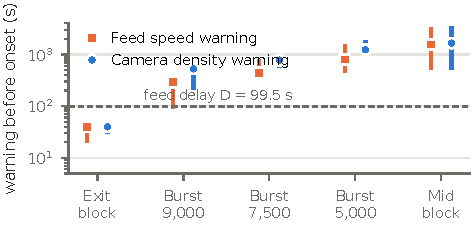
\includegraphics[width=\linewidth]{figs/fig_warning.pdf}
\caption{How early each signal warns: time before the first jam of each no-control run at which the feed's speed fell below 80\% of its pre-trigger level, or the camera's density rose three standard deviations above its own, for 30\,s. Medians and interquartile ranges; dashed: the feed delay $D$.}
\label{fig:warning}
\end{minipage}\hfill
\begin{minipage}[t]{0.485\columnwidth}\centering\vspace{0pt}
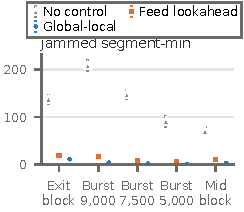
\includegraphics[width=\linewidth]{figs/fig_jams.pdf}
\caption{Jam time by trigger, ordered by how soon no control jams: jammed segment-minutes, mean and two standard errors over 15 seeds.}
\label{fig:jams}
\end{minipage}
\end{figure}

\noindent\textbf{Network.} We evaluate preventive control in the twelve-super-segment Mainz highway model from~\cite{self_regulating_cars}, implemented in SUMO. Its three-to-two-lane exit is the principal breakdown location. To give upstream control time to affect arrivals, rather than injecting vehicles immediately at the network boundary, we extend each of the eight entrances with an unobserved 3\,km approach road. Advisories enter SUMO as speed caps; its car-following model still responds to leading vehicles. The model recorded no collisions in 3,000 controlled runs, without establishing field safety.

\noindent\textbf{Disturbances.} Background demand is fixed at 3,572\,veh/h, above the jammed exit's discharge rate but below free-flow breakdown demand. Consequently, the network remains unjammed without a trigger, yet a queue that forms does not drain under sustained demand (Proposition~\ref{prop:drain}). Fifteen minutes into each two-hour run, we introduce one of five disturbances to vary the available warning time. Three increase total inflow to 5,000\,veh/h for ten minutes or to 7,500 and 9,000\,veh/h for five minutes; without control, breakdown follows after a median 14--28 minutes. Two five-minute lane blockages yield different onset times: 80\,s at the exit versus 37 minutes mid-network. The feed follows the measured Mainz delivery process with $D=99.5$\,s.

\noindent\textbf{Metrics.} A super-segment is jammed when its mean speed is below 19\,km/h, a threshold fitted to the network's speed distribution by the rule of~\cite{bhardwaj2023understanding}, and a jam starts when that state lasts 120\,s. Jam time is the jammed segment-minutes on the twelve super-segments of the network, and a run is jam-free when the network has no jam. Throughput is the flow served at the exit. Travel time is the vehicle-hours all vehicles spend in the network.

\noindent\textbf{Baselines, ablations and protocol.} No control lets every vehicle drive at its own desired speed. The feed lookahead is a rule-based feed-only lookahead baseline: it advises 0.5 of the limit when the next super-segment downstream has a jam factor of 2 or more, and 0.75 when the one after it has. Ablations remove the camera (plan only), the feed and plan (camera only), the gate, or camera error (true occupancy within 60\,m). All use the same 15 seeds at full penetration. Thresholds were chosen on five separate selection seeds, the gate last, as the candidate with the least jam among those costing at most 1\% of throughput beyond the plan alone with no trigger. We report means over seeds and, for differences, the paired mean with two standard errors.

\subsection{The Camera Warns Before the Feed}
\label{sec:warn}

On the three bursts the camera's density warning came first on 43 of 45 runs, by a median of 210 to 480\,s (Fig.~\ref{fig:warning}). The reason is the shape of the speed-density relation: as occupancy rises to 0.05 the median segment speed falls only from 57.5 to 55.0\,km/h, and then to 35.8\,km/h by 0.07. On the exit block the feed's warning was shorter than $D$ on all 15 runs, so by Proposition~\ref{prop:lag} no controller that reads only the feed could change a speed before that jam began.

\subsection{Jams Prevented and Jam Time}
\label{sec:prevent}

Of 75 triggered no-control runs, 74 jammed. The combined system prevents 55 of these jams and reduces mean jam time from 130.8 to 3.9 segment-minutes per run, a 97\% decrease (Table~\ref{tab:main}, Fig.~\ref{fig:jams}). Compared with feed lookahead, it leaves 67\% less jam ($-7.8\pm1.3$ segment-minutes) and serves 9.9\% more traffic. Prevention is not always possible, however: the exit blockage produces breakdown within 80\,s, before the delayed gate can enable local intervention. The system prevents no jams in that case but still reduces jam time from 137.1 to 11.1 segment-minutes. Its benefit thus includes mitigating jams that develop too quickly to prevent.

\subsection{What Each Layer Contributes}
\label{sec:ablation}

The ablations show why the two sensing scales must work together (Table~\ref{tab:main}). The global plan prevents many jams (39 jam-free runs) but cannot prevent breakdown after the largest burst, for which feed observations arrive too late. The camera reacts sooner, yet acting alone it prevents only five jams: without a lower global plan, its single-step correction can reduce a full-limit advisory only to 0.75 of the limit, even though it changes the displayed speed on 32\% of vehicle-ticks. Combining the layers raises the jam-free count to 51 without the gate and 56 with it; replacing camera estimates with true occupancy adds only two further runs. The combined system also serves 3.9\% more traffic ($\pm0.3\%$) while reducing network vehicle-hours by 12.6\% ($\pm1.4\%$). In contrast, feed lookahead loses 5.4\% throughput because its response to downstream slowdown is applied upstream without checking local traffic conditions.

\subsection{The Cost When No Jam Would Form}
\label{sec:notrigger}

Early intervention is beneficial only when it is selective. Even without a disturbance, near-capacity traffic often produces occupancy close to $k_c$, causing the ungated local rule to reduce speed unnecessarily. In no-trigger runs, this reduces throughput by 6.9\% relative to no control, compared with 2.9\% for the plan alone. Replacing the camera with true occupancy still incurs a 5.9\% penalty, indicating that the main problem is the trigger rule rather than measurement noise. The feed gate reduces corrected vehicle-ticks from 15.5\% to 0.2\% and limits the throughput penalty to 3.0\%. Allowing occupancy itself to open the gate at $\hat k\ge0.8k_c$ or $k_c$ violated the selection criterion; releasing correction while traffic discharged offered negligible benefit. However, using the delayed feed to suppress false alarms also creates a blind spot: on the rapid exit-block disturbance, the gate activates too late and adds $3.0\pm0.9$ jammed segment-minutes relative to no gate.

\subsection{Partial Compliance and Driver Response}
\label{sec:sens}

\begin{figure}[t]
\centering
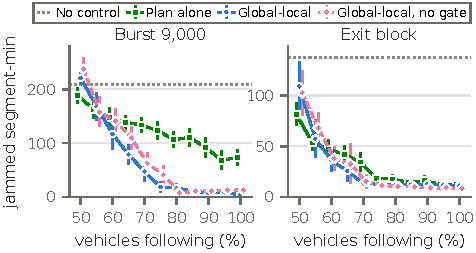
\includegraphics[width=\linewidth]{figs/fig_penetration.pdf}
\caption{Jam time against the share of vehicles that follow the advice, on the largest burst and the exit block: jammed segment-minutes, mean and two standard errors over 15 seeds. No control is the dotted line.}
\label{fig:penetration}
\end{figure}

\noindent\textbf{Share of drivers who follow.} Because an advisory cannot regulate vehicles whose drivers ignore it, we vary participation on the largest burst and the exit-block disturbance (Fig.~\ref{fig:penetration}). The exit-block case improves over no control at every tested share, whereas the largest burst requires at least 55\% participation. At 75\%, the gate reduces burst jam time to 18.5 segment-minutes, compared with 41.4 without it. At 50\%, the combined policy instead exceeds no control by $13.0\pm15.9$ segment-minutes, although this is smaller than the $29.5\pm24.6$ excess without the gate; it also exceeds the plan alone by $32.6\pm17.2$. Releasing the correction during queue discharge does not eliminate the degradation ($+13.1\pm21.3$). Thus, the local correction's benefit is conditional on sufficient participation, not merely on its early warning.

\noindent\textbf{Driver response.} Participation is only part of compliance: even drivers who heed an advisory may react late or exceed its recommended speed. We therefore model a lognormal reaction delay, a positive speed offset, and bounded deceleration, using assumed parameters because the field drives did not test human response. Nominal drivers react in a median 2\,s, with $5\pm5\%$ offset and 1.5\,m/s$^2$ deceleration; lax drivers take 4\,s, with $15\pm10\%$ and 1.0\,m/s$^2$. This distinction matters most during the largest burst: jam time rises from 3.7 segment-minutes with exact compliance to 11.1 nominally and 46.7 with lax response. The exit block is less sensitive (11.1, 12.3, and 13.7, respectively). Both groups outperform no control and plan-only under corresponding responses on every seed, but the burst sensitivity motivates measuring driver behavior before field claims.

\noindent\textbf{Camera scale and feed delay.} The two sensing assumptions affect performance differently. Scaling camera distances by 0.8 or 1.25 changes jam time by at most 1.8 segment-minutes, and the gated system remains better than feed lookahead; without the gate, the 0.8-scale burst produces $25.0\pm15.9$ more segment-minutes than lookahead. Feed delay has a more structural effect because it also postpones gate activation. On the exit block, the combined policy beats lookahead at $D=0$, 189, and 368\,s. On the burst it does so at $D=0$, but at 189 and 368\,s the differences are small relative to uncertainty ($+2.9\pm10.8$ and $-0.8\pm5.3$). At those two delays, ungated jam times are 4.9 and 6.8 segment-minutes, compared with 14.5 and 17.5 with the gate. The gate that prevents unnecessary slowing can therefore become the limiting factor when the global feed is substantially delayed.



\section{Conclusion and Limitations}
\label{sec:conclusion}

Version-keyed planning coordinates decentralized advisories from delayed network feeds, while a gated camera correction responds to rising local occupancy. Together, the layers reduced simulated Mainz jam time by 97\% and increased throughput by 3.9\% under disturbances. Neither layer alone achieved the same performance, while ungated corrections increased unnecessary slowing.

Whether these gains transfer to human-driven traffic remains open. Road tests established that advisories can be computed onboard, not that drivers respond sufficiently quickly or consistently. Because partial compliance weakens control in the largest burst, approved closed-course response and safety studies should precede fleet trials measuring traffic outcomes.

Beyond uncertainty in driver response, the gate introduces an algorithmic challenge: it prevents unnecessary slowing but can suppress visual intervention during rapid breakdown while awaiting the feed. A local trigger that distinguishes incipient jams from harmless high occupancy could remove that dependence. Testing it across networks and longer feed traces would establish whether this tradeoff generalizes.


\begin{thebibliography}{10}
\providecommand{\url}[1]{#1}
\csname url@rmstyle\endcsname
\providecommand{\newblock}{\relax}
\providecommand{\bibinfo}[2]{#2}
\providecommand\BIBentrySTDinterwordspacing{\spaceskip=0pt\relax}
\providecommand\BIBentryALTinterwordstretchfactor{4}
\providecommand\BIBentryALTinterwordspacing{\spaceskip=\fontdimen2\font plus
\BIBentryALTinterwordstretchfactor\fontdimen3\font minus
  \fontdimen4\font\relax}
\providecommand\BIBforeignlanguage[2]{{%
\expandafter\ifx\csname l@#1\endcsname\relax
\typeout{** WARNING: IEEEtran.bst: No hyphenation pattern has been}%
\typeout{** loaded for the language `#1'. Using the pattern for}%
\typeout{** the default language instead.}%
\else
\language=\csname l@#1\endcsname
\fi
#2}}

\bibitem{bhardwaj2023understanding}
A.~Bhardwaj, S.~R. Iyer, S.~Ramesh, J.~White, and L.~Subramanian,
  ``Understanding sudden traffic jams: From emergence to impact,''
  \emph{Development Engineering}, vol.~8, p. 100105, 2023.

\bibitem{papageorgiou2002freeway}
M.~Papageorgiou and A.~Kotsialos, ``Freeway ramp metering: An overview,''
  \emph{IEEE transactions on intelligent transportation systems}, vol.~3,
  no.~4, pp. 271--281, 2002.

\bibitem{hegyi2008specialist}
A.~Hegyi, S.~P. Hoogendoorn, M.~Schreuder, H.~Stoelhorst, and F.~Viti,
  ``{SPECIALIST}: A dynamic speed limit control algorithm based on shock wave
  theory,'' in \emph{Proceedings of the 11th International IEEE Conference on
  Intelligent Transportation Systems (ITSC)}, 2008, pp. 827--832.

\bibitem{lee2024traffic}
{CIRCLES Consortium}, ``Traffic control via connected and automated vehicles:
  An open-road field experiment with 100 cavs,'' \emph{arXiv preprint
  arXiv:2402.17043}, 2024.

\bibitem{wang2018latency}
Z.~Wang, M.~Hamedi, E.~Sharifi, and S.~Young, ``A cross-vendor and cross-state
  analysis of the {GPS}-probe data latency,'' \emph{Transportation Research
  Record}, vol. 2672, no.~42, pp. 180--191, 2018.

\bibitem{self_regulating_cars}
A.~Bhardwaj, R.~Asim, S.~K. Chauhan, Y.~Zaki, and L.~Subramanian,
  ``Self-regulating cars: Automating traffic control in free flow road
  networks,'' in \emph{Proceedings of the AAAI Conference on Artificial
  Intelligence}, 2026.

\bibitem{arnold1998ramp}
E.~D. Arnold, Jr., ``Ramp metering: a review of the literature.'' Virginia
  Transportation Research Council, Tech. Rep., 1998.

\bibitem{li2017reinforcement}
Z.~Li, P.~Liu, C.~Xu, H.~Duan, and W.~Wang, ``Reinforcement learning-based
  variable speed limit control strategy to reduce traffic congestion at freeway
  recurrent bottlenecks,'' \emph{IEEE transactions on intelligent
  transportation systems}, vol.~18, no.~11, pp. 3204--3217, 2017.

\bibitem{hegyi2013cooperative}
A.~Hegyi, \emph{et~al.}, ``A cooperative system based variable speed limit
  control algorithm against jam waves -- an extension of the {SPECIALIST}
  algorithm,'' in \emph{Proceedings of the 16th International IEEE Conference
  on Intelligent Transportation Systems (ITSC)}, 2013, pp. 973--978.

\bibitem{stern2018dissipation}
R.~E. Stern, \emph{et~al.}, ``Dissipation of stop-and-go waves via control of
  autonomous vehicles: Field experiments,'' \emph{Transportation Research Part
  C: Emerging Technologies}, vol.~89, pp. 205--221, 2018.

\bibitem{wu2017flow}
C.~Wu, A.~Kreidieh, K.~Parvate, E.~Vinitsky, and A.~M. Bayen, ``Flow: A modular
  learning framework for mixed autonomy traffic,'' \emph{arXiv preprint
  arXiv:1710.05465}, 2017.

\bibitem{vinitsky2018benchmarks}
E.~Vinitsky, A.~Kreidieh, L.~L. Flem, N.~Kheterpal, K.~Jang, F.~Wu, C.~Wu,
  R.~Liaw, E.~Liang, and A.~M. Bayen, ``Benchmarks for reinforcement learning
  in mixed-autonomy traffic,'' in \emph{Proceedings of the 2nd Conference on
  Robot Learning}.\hskip 1em plus 0.5em minus 0.4em\relax PMLR, 2018, pp.
  399--409.

\bibitem{kreidieh2018dissipating}
A.~R. Kreidieh, C.~Wu, and A.~M. Bayen, ``Dissipating stop-and-go waves in
  closed and open networks via deep reinforcement learning,'' in \emph{2018
  21st International Conference on Intelligent Transportation Systems
  (ITSC)}.\hskip 1em plus 0.5em minus 0.4em\relax IEEE, 2018, pp. 1475--1480.

\bibitem{cho2023temporal}
J.-H. Cho, S.~Li, J.~Kim, and C.~Wu, ``Temporal transfer learning for traffic
  optimization with coarse-grained advisory autonomy,'' \emph{arXiv preprint
  arXiv:2312.09436}, 2023.

\bibitem{herrera2010evaluation}
J.~C. Herrera, D.~B. Work, R.~Herring, X.~Ban, Q.~Jacobson, and A.~M. Bayen,
  ``Evaluation of traffic data obtained via {GPS}-enabled mobile phones: The
  {Mobile Century} field experiment,'' \emph{Transportation Research Part C:
  Emerging Technologies}, vol.~18, no.~4, pp. 568--583, 2010.

\bibitem{seo2017traffic}
T.~Seo, A.~M. Bayen, T.~Kusakabe, and Y.~Asakura, ``Traffic state estimation on
  highway: A comprehensive survey,'' \emph{Annual Reviews in Control}, vol.~43,
  pp. 128--151, 2017.

\bibitem{nayyar2013common}
A.~Nayyar, A.~Mahajan, and D.~Teneketzis, ``Decentralized stochastic control
  with partial history sharing: A common information approach,'' \emph{IEEE
  Transactions on Automatic Control}, vol.~58, no.~7, pp. 1644--1658, 2013.

\bibitem{kenney2011dedicated}
J.~B. Kenney, ``Dedicated short-range communications ({DSRC}) standards in the
  united states,'' \emph{Proceedings of the IEEE}, vol.~99, no.~7, pp.
  1162--1182, 2011.

\bibitem{sae2020j2735}
{SAE International}, ``{V2X} communications message set dictionary,'' SAE
  International, Tech. Rep. J2735, 2020.

\bibitem{here_traffic_api}
{HERE Technologies}, ``{HERE} traffic {API} v7 developer guide,''
  \url{https://www.here.com/docs/bundle/traffic-api-v7-api-reference}, 2025,
  accessed: 2026-09-12.

\bibitem{auxer2007rating}
G.~A. Auxer, J.~F. Carroll, and B.~J. Smyth, ``Rating that represents the
  status along a specified driving route,'' U.S. Patent 7,302,341 B1, Nov.
  2007.

\bibitem{redmon2016yolo}
J.~Redmon, S.~Divvala, R.~Girshick, and A.~Farhadi, ``You only look once:
  Unified, real-time object detection,'' in \emph{Proceedings of the IEEE
  Conference on Computer Vision and Pattern Recognition (CVPR)}, 2016, pp.
  779--788.

\end{thebibliography}

\end{document}
